\documentclass[a4paper]{article}

\usepackage{hyperref}
%\hypersetup{
%colorlinks=false,              % bool: Liens colorés
%pdfborder={0 0 0}             % Ne pas encadrer les liens
%}
\usepackage[utf8]{inputenc}  
\usepackage[francais]{babel}  
\usepackage[top=2cm, bottom=2cm, left=2cm, right=2cm]{geometry}
\usepackage{graphicx}
\usepackage[final]{pdfpages} 
\usepackage{rotating}
\usepackage{eurosym}
\usepackage{lscape}
\usepackage{float}
% définir les commandes ici

% s'il y a beaucoup de commandes et de packages à inclure n'h&ésitez pas
% à mettre tout ça dans un fichier include.tex et l'inclure
% \input{include.tex}


\begin{document}

%------------------------------------- Page de titre
\begin{titlepage}
~ 
\vfill
	\begin{center}
		\begin{Huge}
		SOA : Dossier de conception d'ensemble\\
		\end{Huge} 
\vfill
		\textbf{Hexanome 4211 :} 
		\\Sandra \bsc{Mondain}, Elisa \bsc{Abidh}, 
		\\Gaël \bsc{Motte}, Armand \bsc{Rossius}, 
		\\Rémi \bsc{Fradet}, Nicolas \bsc{Silva}, Julien \bsc{Levesy}\\

\vfill		
		\begin{Large}
		Avril 2011
		\end{Large}
\vfill

	\end{center}
\vfill
\end{titlepage}
%----------------------------------------------------

%--------------------------------- Table des matières
\newpage
\tableofcontents
\newpage
%----------------------------------------------- Plan

\section*{Intro}
\\
\\
\\
\\
\\
\\
\\
\section{Diagrammes d'Activité}
Todo : importer ici les pnggénérés par cacoo
\section{Découpage en Blocs}
\begin{figure}[H]
	\begin{center}
	% l b r t
		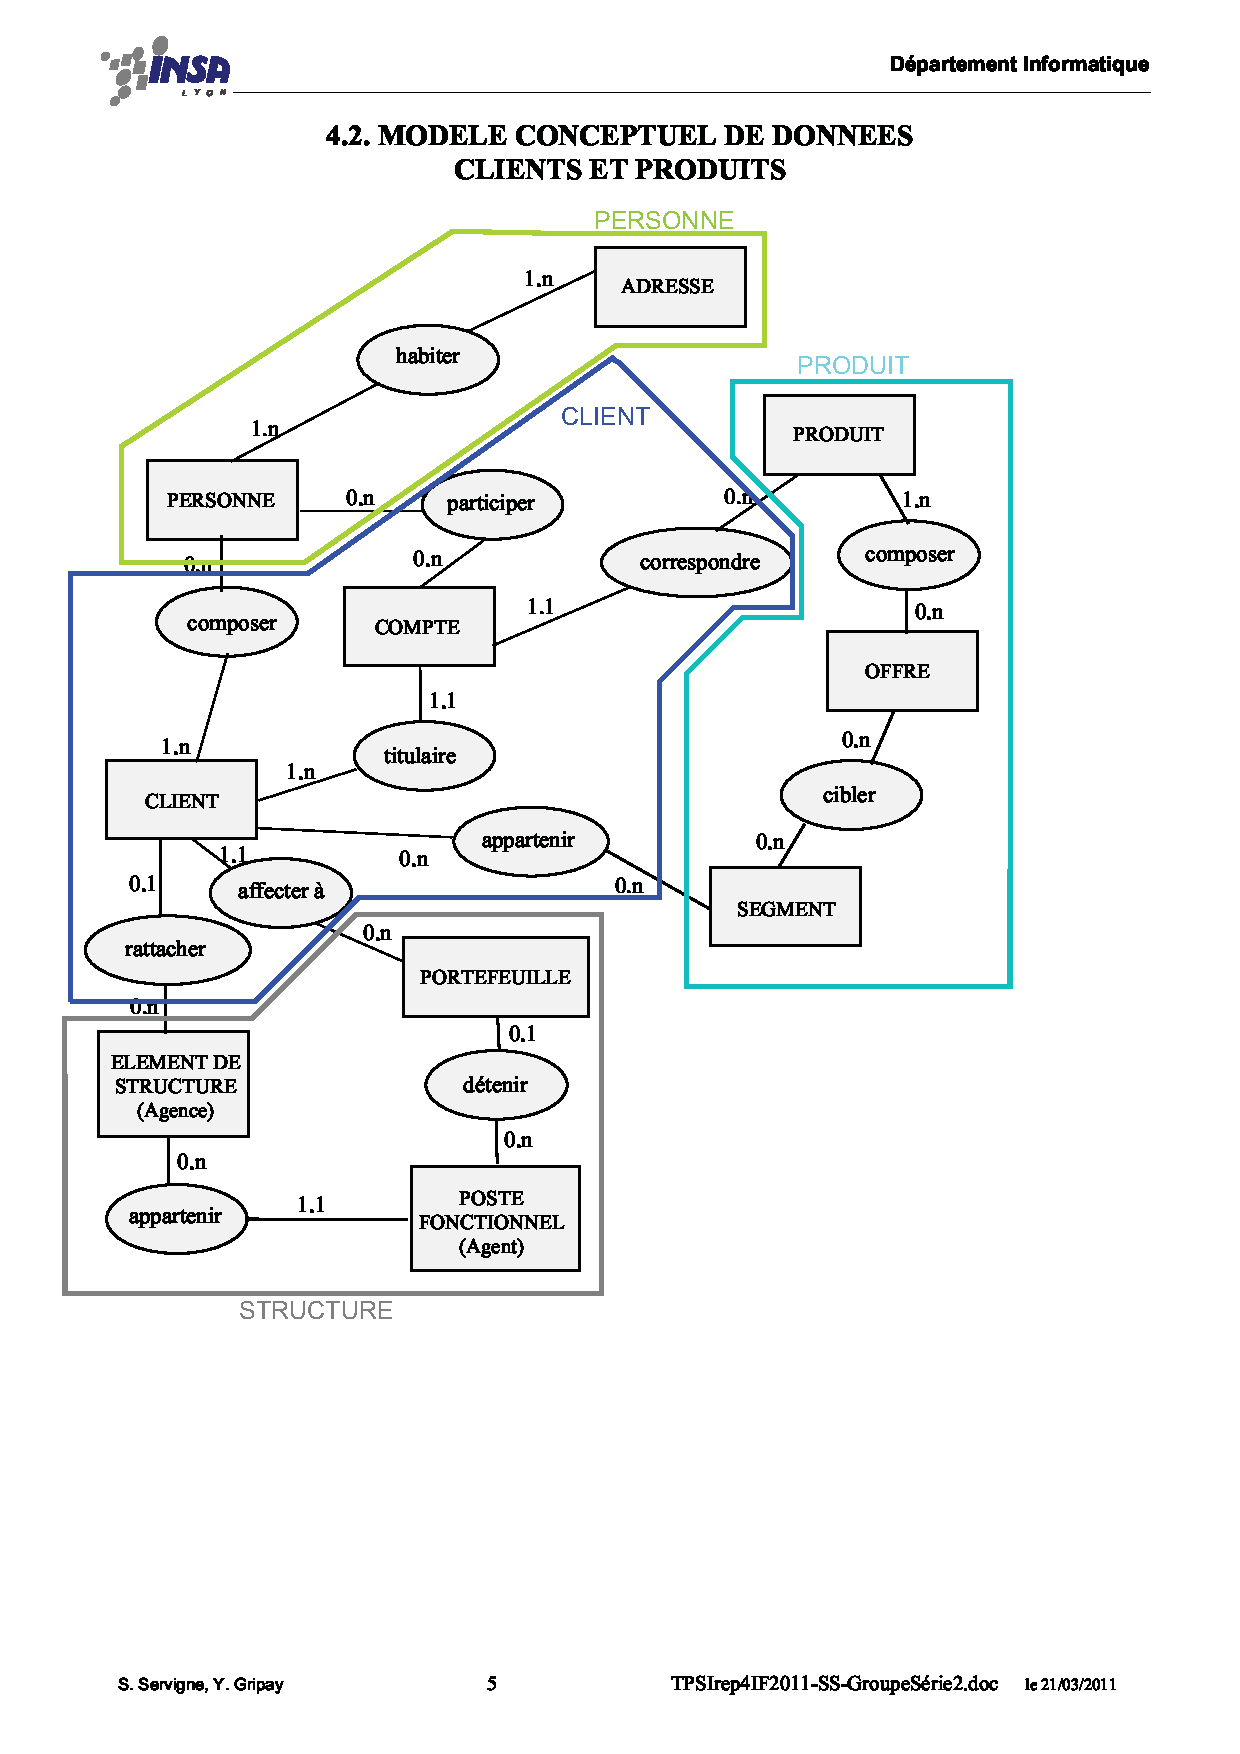
\includegraphics[scale=0.8,clip, trim = 5mm 65mm 35mm 35mm]{Includes/SOA-Blocs-1.pdf}
		\caption{Découpage en bloc du MCD Clients et Produits}
	\end{center}
\end{figure}

\begin{figure}[H]
	\begin{center}
		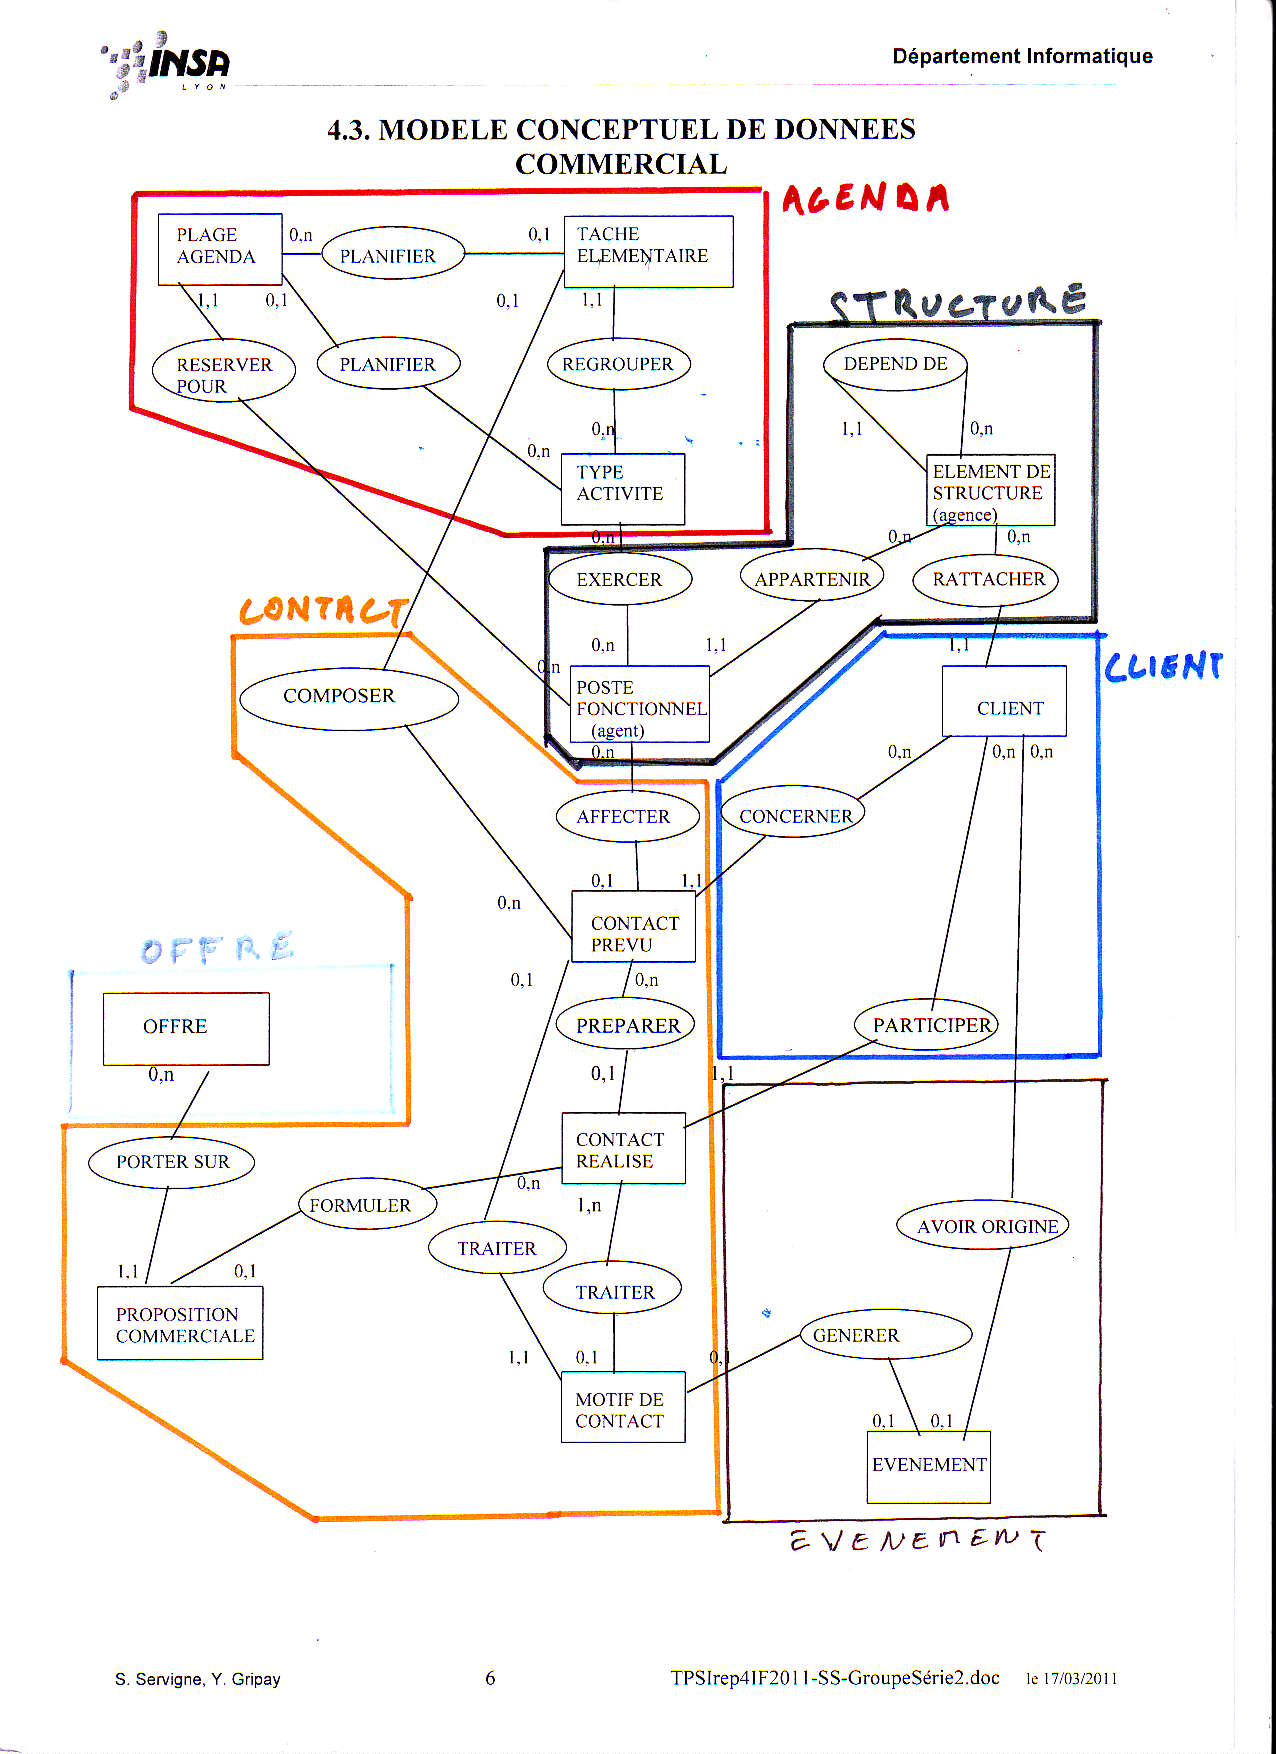
\includegraphics[scale=0.8,clip, trim = 5mm 30mm 3mm 30mm]{Includes/SOA-Blocs-2.pdf}
		\caption{Découpage en bloc du MCD Commercial}
	\end{center}
\end{figure}

\section{Diagrammes de Séquences}

\begin{figure}[H]
	\begin{center}
		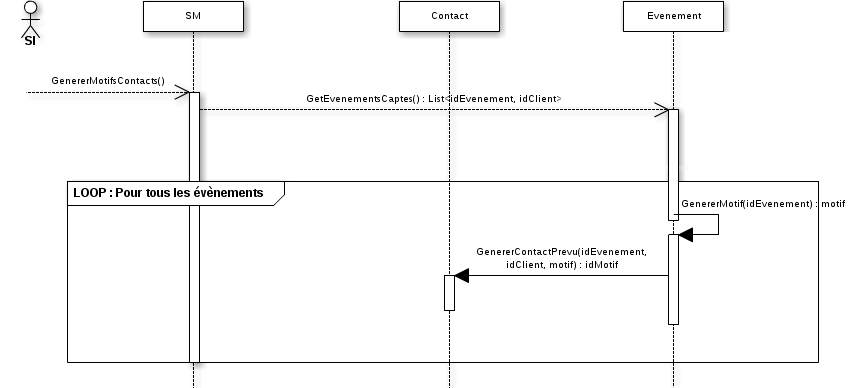
\includegraphics[scale=0.4]{Includes/SOA-Sequence-CU1.png}
		\caption{Diagramme de séquence pour le CU1}
	\end{center}
\end{figure}

\begin{figure}[H]
	\begin{center}
		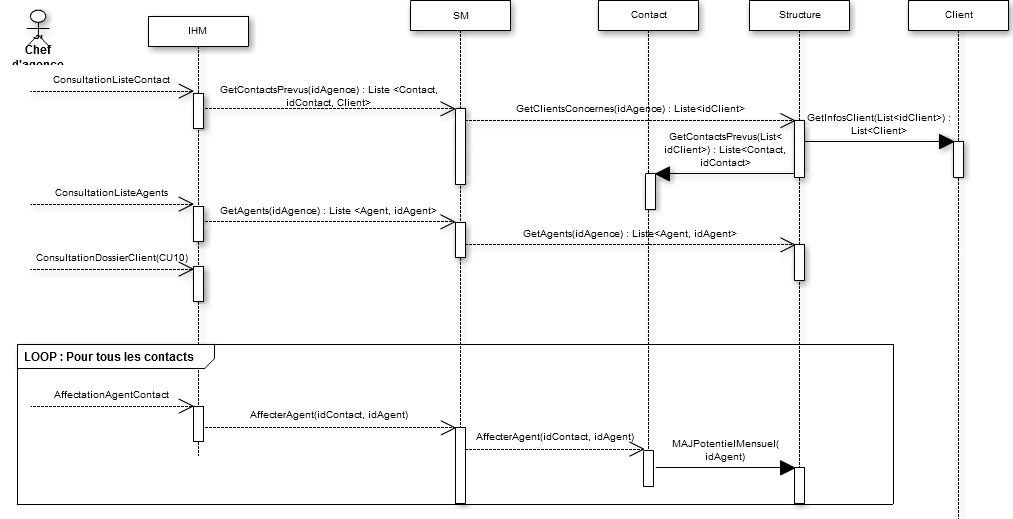
\includegraphics[scale=0.4]{Includes/SOA-Sequence-CU2.png}
		\caption{Diagramme de séquence pour le CU2}
	\end{center}
\end{figure}

\begin{figure}[H]
	\begin{center}
		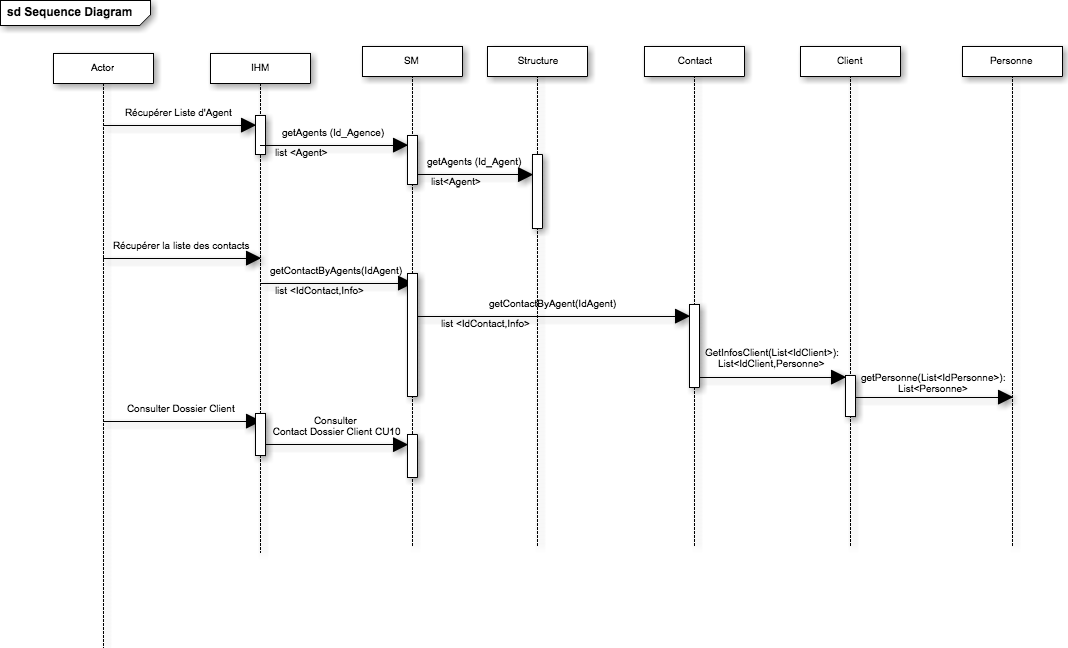
\includegraphics[scale=0.4]{Includes/SOA-Sequence-CU3.png}
		\caption{Diagramme de séquence pour le CU3}
	\end{center}
\end{figure}

\begin{figure}[H]
	\begin{center}
		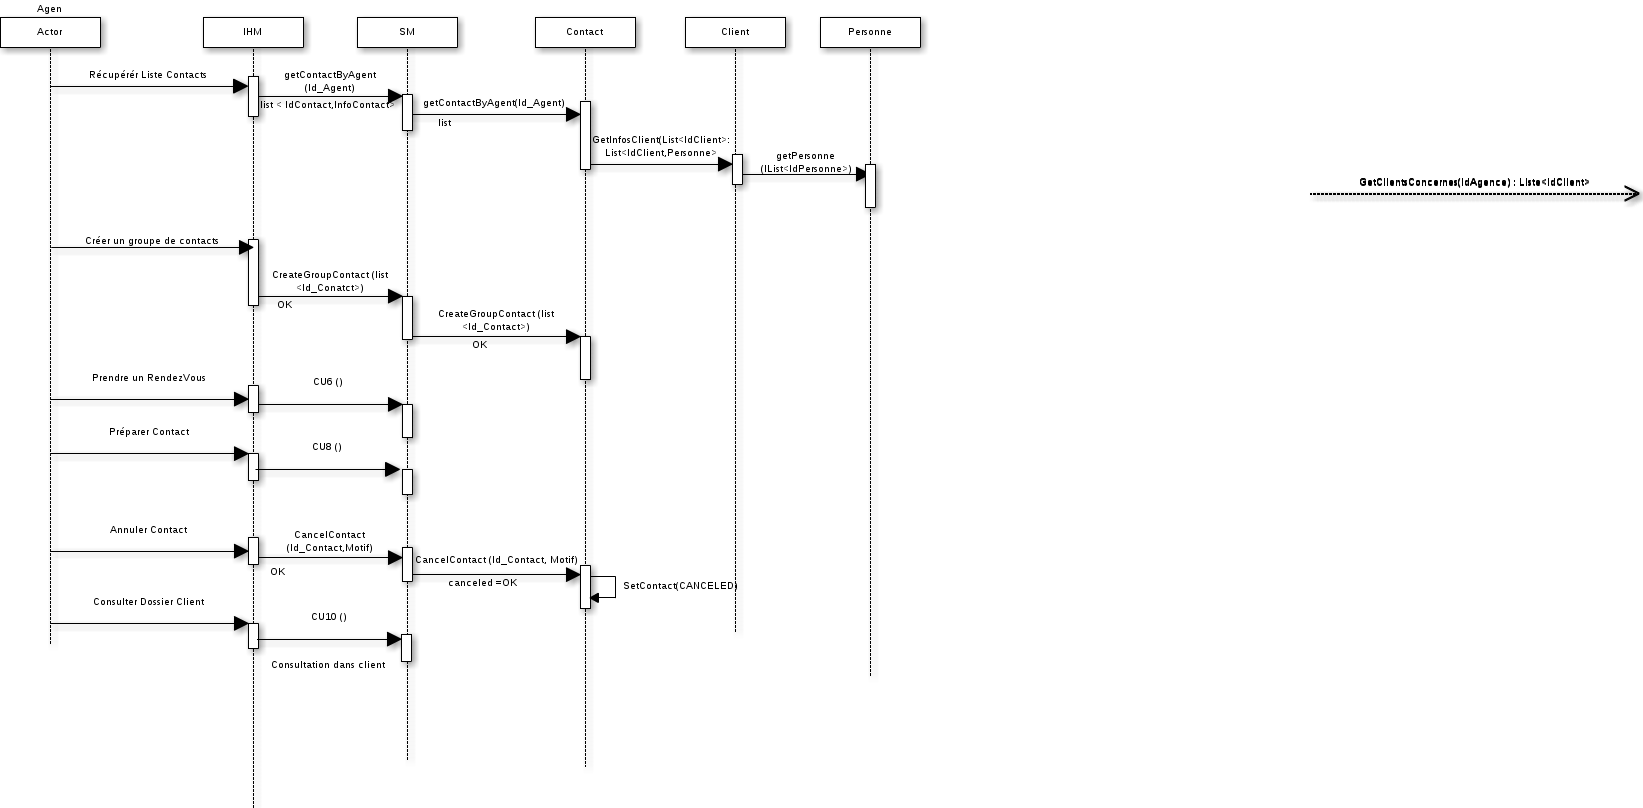
\includegraphics[scale=0.4]{Includes/SOA-Sequence-CU4.png}
		\caption{Diagramme de séquence pour le CU4}
	\end{center}
\end{figure}

\begin{figure}[H]
	\begin{center}
		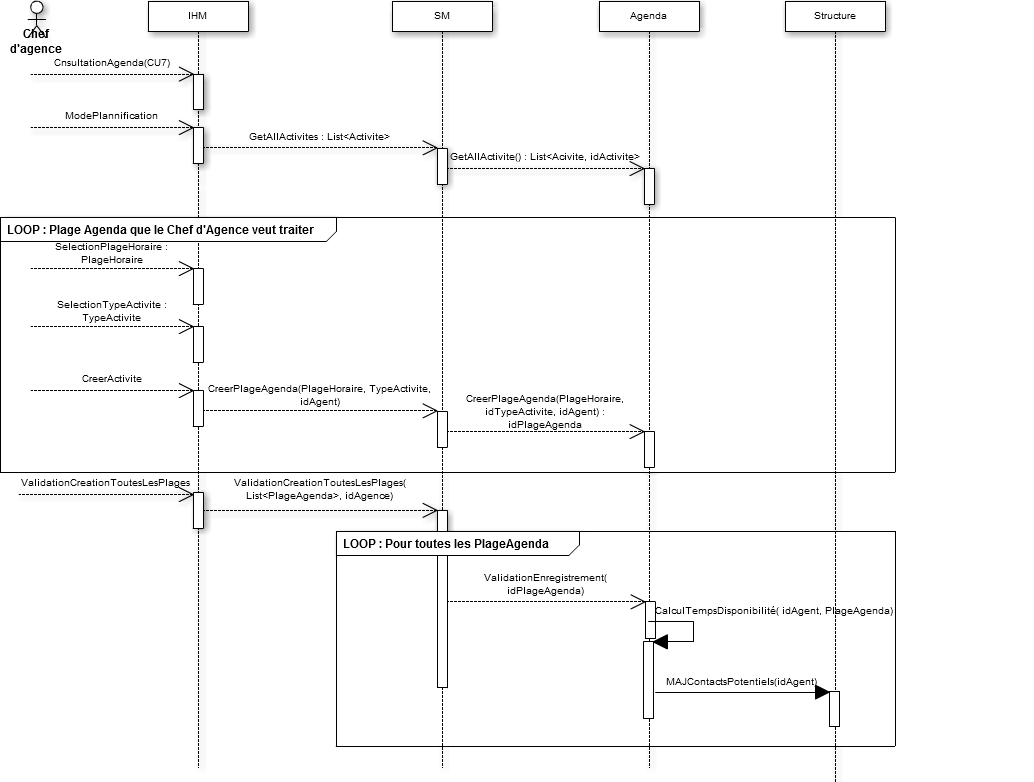
\includegraphics[scale=0.4]{Includes/SOA-Sequence-CU5.png}
		\caption{Diagramme de séquence pour le CU5}
	\end{center}
\end{figure}



\begin{figure}[H]
	\begin{center}
		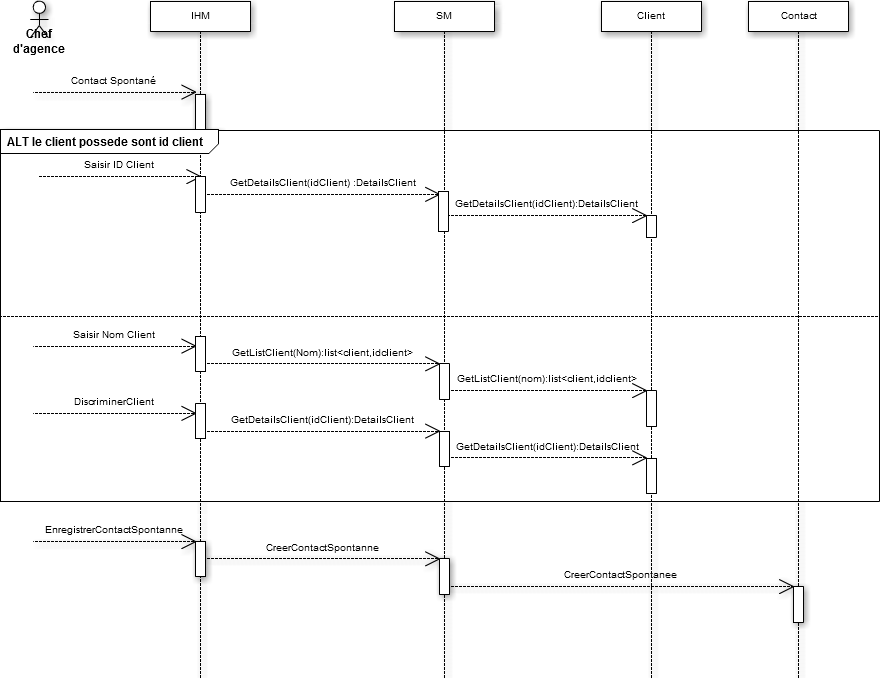
\includegraphics[scale=0.4]{Includes/SOA-Sequence-CU6-a.png}
		\caption{Diagramme de séquence pour le CU6-a}
	\end{center}
\end{figure}
\begin{figure}[H]
	\begin{center}
		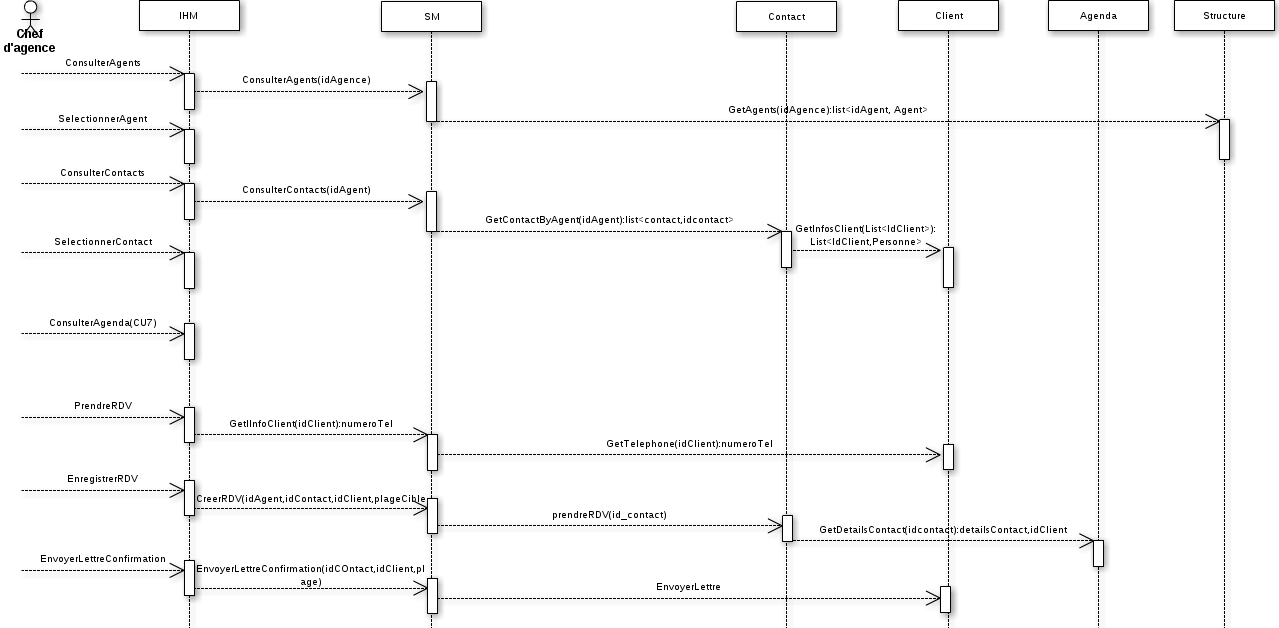
\includegraphics[scale=0.4]{Includes/SOA-Sequence-CU6-b.png}
		\caption{Diagramme de séquence pour le CU6-b}
	\end{center}
\end{figure}

\begin{figure}[H]
	\begin{center}
		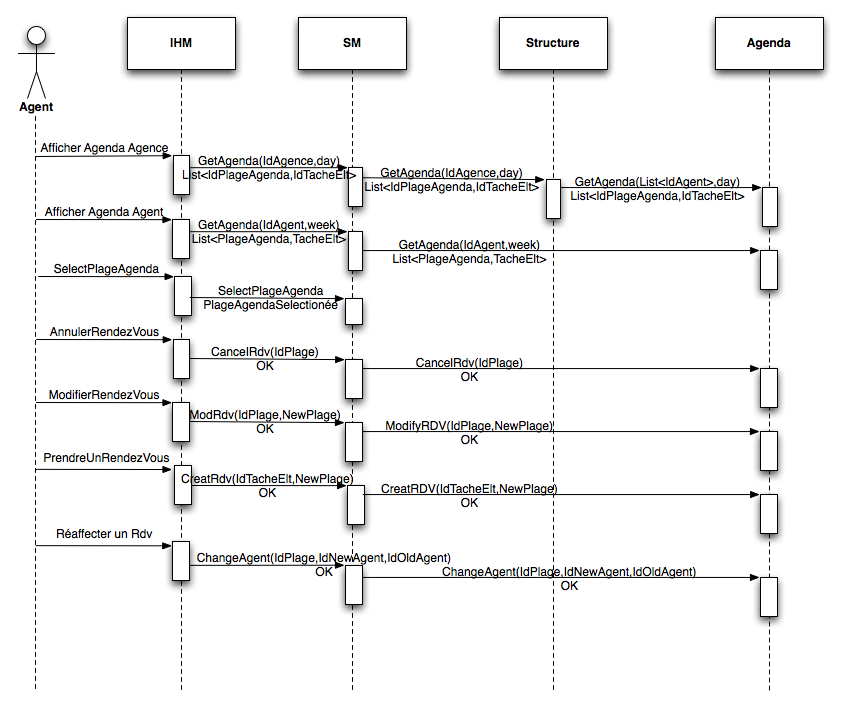
\includegraphics[scale=0.4]{Includes/SOA-Sequence-CU7.png}
		\caption{Diagramme de séquence pour le CU7}
	\end{center}
\end{figure}

\begin{figure}[H]
	\begin{center}
		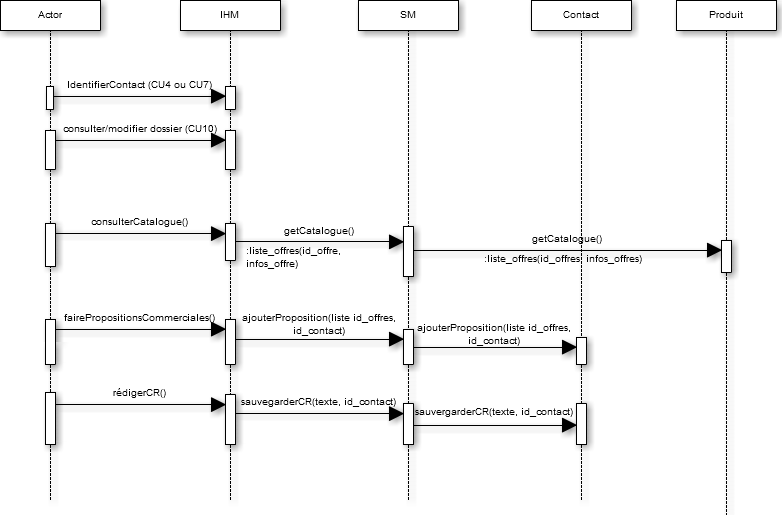
\includegraphics[scale=0.4]{Includes/SOA-Sequence-CU8.png}
		\caption{Diagramme de séquence pour le CU8}
	\end{center}
\end{figure}

\begin{figure}[H]
	\begin{center}
		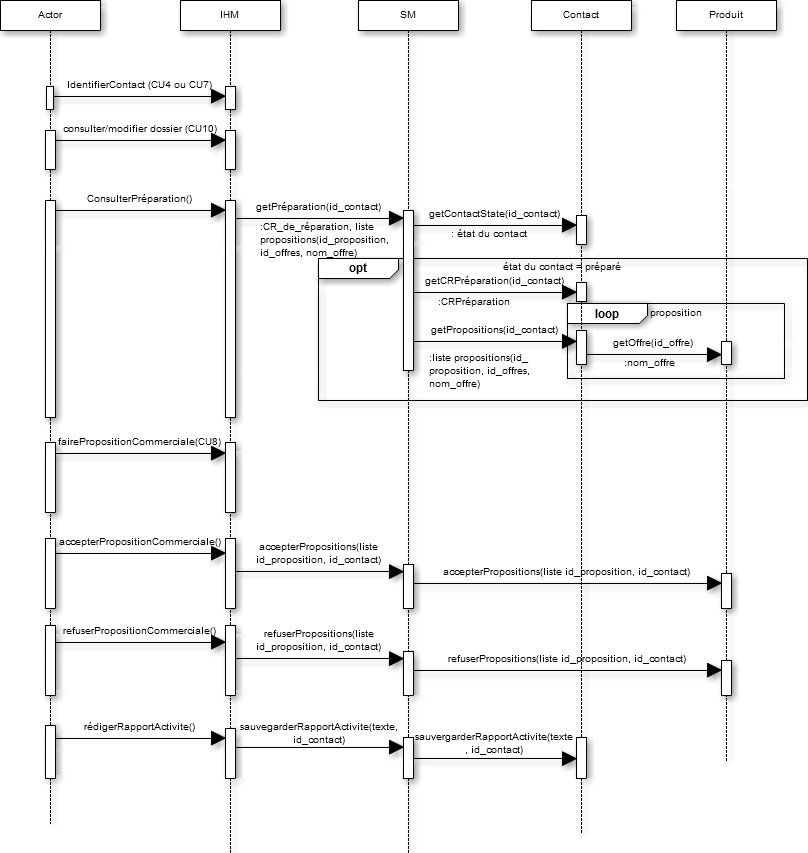
\includegraphics[scale=0.4]{Includes/SOA-Sequence-CU9.png}
		\caption{Diagramme de séquence pour le CU9}
	\end{center}
\end{figure}

\begin{figure}[H]
	\begin{center}
		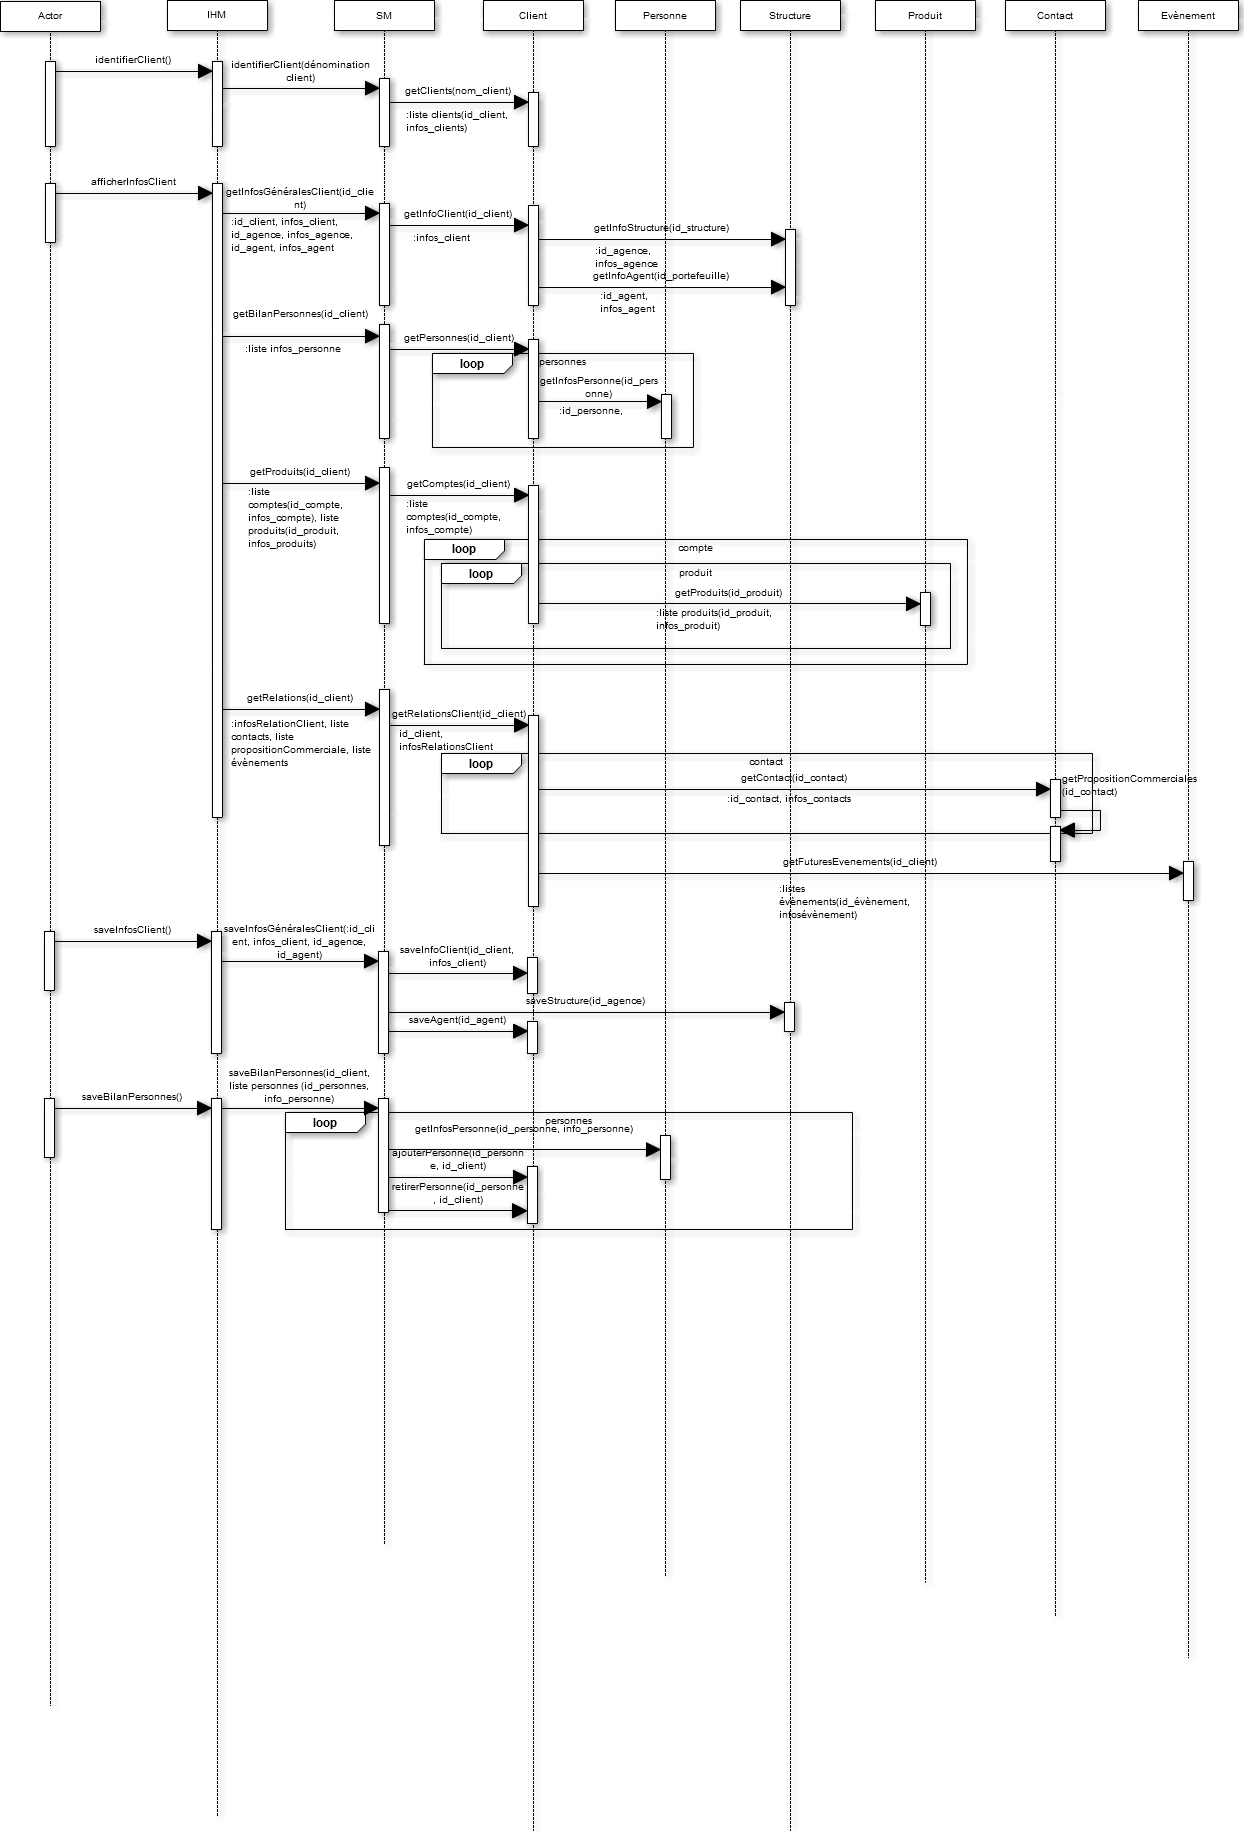
\includegraphics[scale=0.4]{Includes/SOA-Sequence-CU10.png}
		\caption{Diagramme de séquence pour le CU10}
	\end{center}
\end{figure}

\section{Diagramme de Collaboration}

\begin{figure}[H]
	\begin{center}
		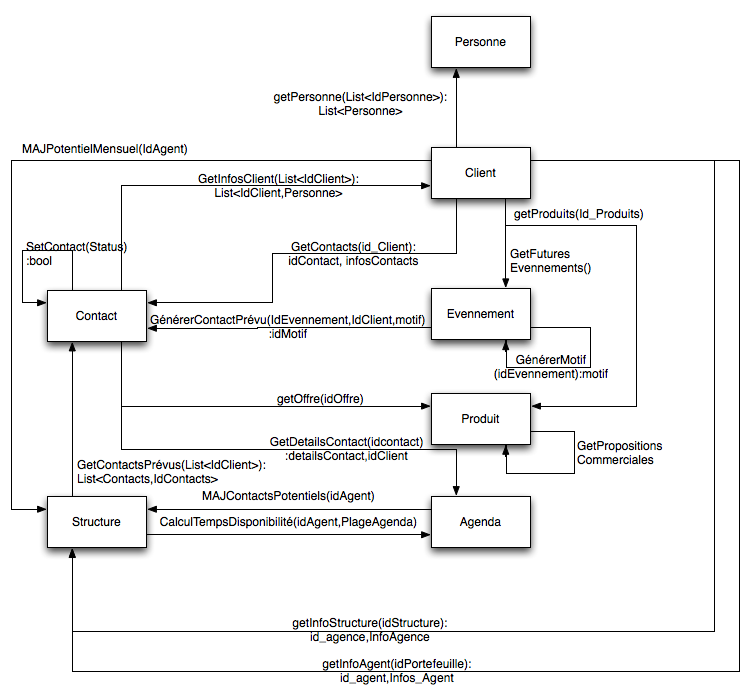
\includegraphics[scale=0.4]{Includes/COLLAB.png}
		\caption{Diagramme de collaboration}
	\end{center}
\end{figure}


\section*{Conclusion}



\end{document}
